%! Author = adam
%! Date = 28.02.21


\chapter{More Ion-Matter Interactions}\label{ch:more-ion-matter-interactions}
In the previous chapter, we covered the basics of ion-matter interactions.
This included the short- and long-range interaction of atoms and what forces govern in the various regimes, followed by the screening potential due to electrons.
Then we covered collisions of atoms and the scattering that occurs therewith.
Now we turn our attention to the following subjects:
\begin{myitemize}
	\item Ion stopping
	\item Energy loss processes
	\item Nuclear Stopping
	\item Electronic Stopping
\end{myitemize}

We want to now understand what it takes to stop an ion as it travels through a medium, as well as how to measure this quantity and receive valuable information therewith.
The application of ion stopping is important in areas such as radiation protection, ion implantation and nuclear medicine.

\section{Ion Stopping}\label{sec:ion-stopping}
The stopping power is a retarding force acting on charged particles due to the interaction with matter resulting in a loss of particle energy.
The stopping power $S$ can be written as the energy loss per unit length:
\begin{equation}
S(E) = -\frac{dE}{dx}\label{eq:stopping}
\end{equation}
and takes on a value of $\approx 100$ eV/mm (in SI units it is Newtons).
The penetration depth $R$ can be then calculated using $E_0$ the initial kinetic energy of the particle:
\begin{equation}
R = \int_0^{E_0} \frac{1}{S(E)}dE
\end{equation}
A way to visualize this is to imagine an ion scattering within a sample, and each time it collides randomly, it is deflected and travels a distance $r_i$ before randomly colliding again, traveling a new distance $r_i$. $R$ is then $R = \sum_i r_i$.
There are two main different energy loss processes that can stop an ion that we will consider.
In nuclear stopping, we have large discrete energy losses for each collision that result in significant angular deflection.
For electronic, there is much smaller energy loss per collision, and negligible deflection.
Together we get the following inelastic collision formula:
This can be seen in Figure~\ref{fig:ionstop}
$$ \frac{dE}{dx} = \frac{dE}{dx} |_n + \frac{dE}{dx}|_e $$
We can further define the \textit{stopping cross section} as $$S_n = \frac{dE}{dx} / N$$ where $N$ is the atomic density and $S_n$ has units of [eVcm$^2$/atom].
This quantity can be understood as the energy loss rate per scattering center.
At low ion energies (low frequency of ion), nuclear stopping dominates, but as we reach higher impact particle energies, we electric stopping dominates.

\begin{figure}
	\centering
	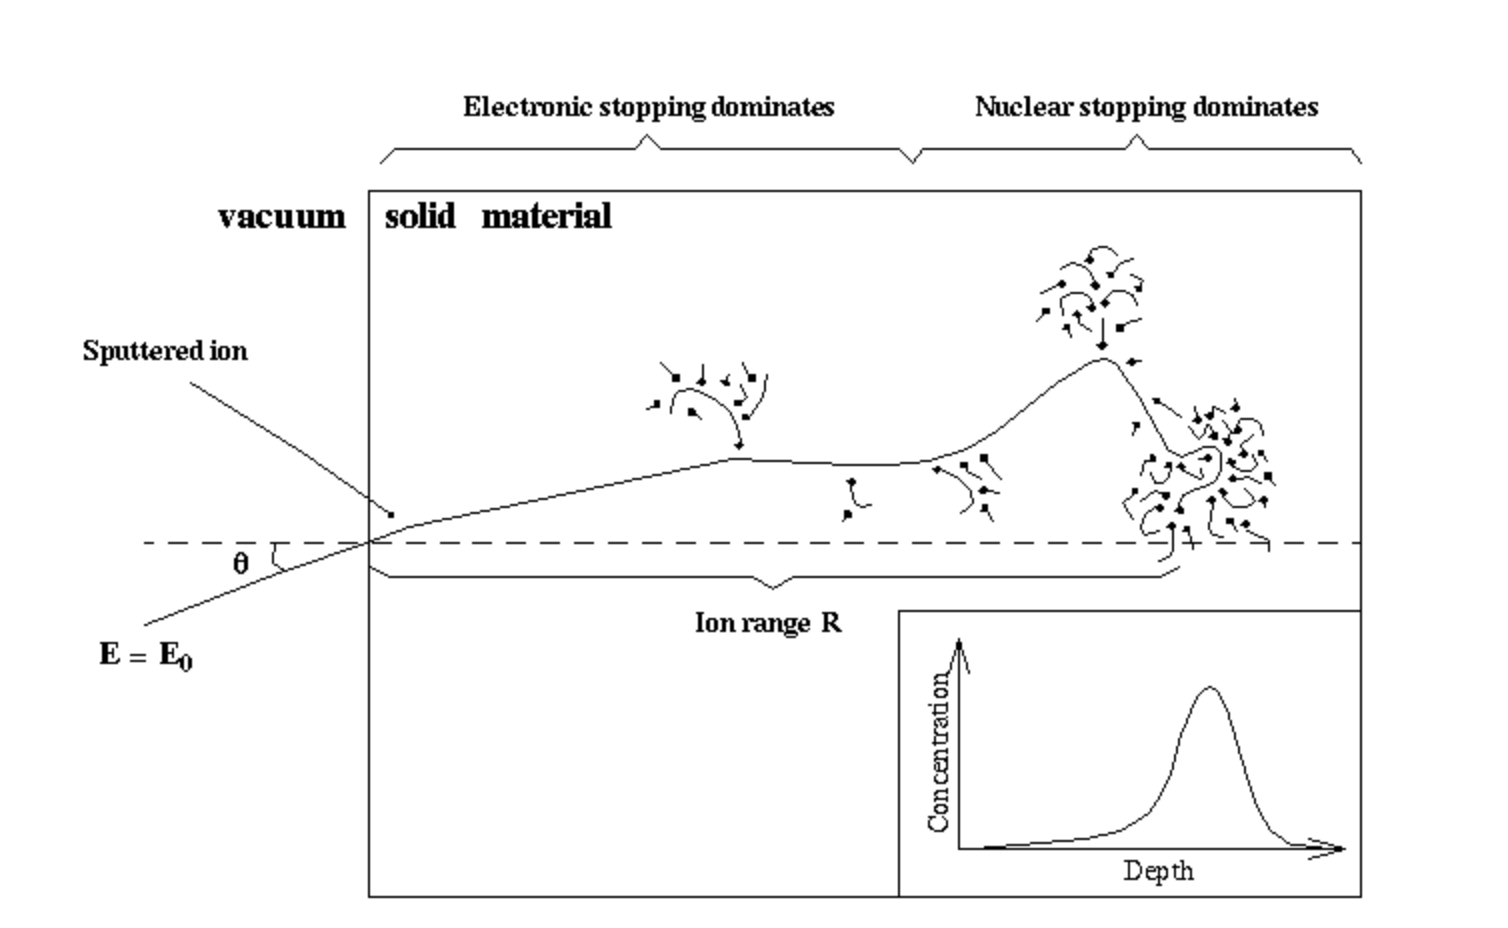
\includegraphics[width=0.6\linewidth, height=6cm]{ionstopping}
	\caption{General picture of ion stopping. Sputtering will be covered in the future.  In the beginning of the slowing down process at high energies, the ion slows down mainly by electronic stopping, and moves almost in a straight path. When the ion has slowed down sufficiently, the collisions with nuclei become more and more probable, finally dominating the slowing down. \cite{4}}
	\label{fig:ionstop}
\end{figure}

\section{Nuclear Stopping}\label{sec:nuclear-stopping}
Nuclear stopping power or the nuclear energy loss rate is the energy loss by a moving ion due to elastic collisions per unit length traveled within the target.
The word nuclear may cause confusion because nuclear stopping is not in fact due to the nuclear forces, but rather is meant to note that this stopping involves the interaction of the ion with the nuclei in the target.
We can then calculated the average energy loss using the probability of a collision for a given energy range: $$ \langle dE \rangle = \int T \frac{dP(E)}{dT}dT = N \int_{T_{min}}^{T_{max}} T \frac{d\sigma (E)}{dT}dTdx$$
For infinitesimal $dx$ we receive the nuclear stopping power $$ \frac{dE}{dx} |_n = N \int_{T_{min}}^{T_{max}} T\frac{d\sigma(E)}{dT}dT$$ where $T_m$ is defined in previous chapters and is the maximum energy transfer.
Using the nuclear stopping power defined above, we can easily calculate the nuclear stopping cross section $S_{nn}$ is defined similarly as before.

\begin{equation}
	S_{nn} = \frac{1}{N} \frac{dE}{dx}|_n = \int_{T_{min}}^{T_{M}} T \underbrace{\frac{d\sigma (E)}{dT}}_\textrm{ETDCS} dT
\end{equation}

The term ETDCS stands for energy transfer differential cross section.
\subsection{ZBL Model}\label{subsec:zbl-model}
To model the nuclear stopping cross section $S_{nn}$, we can use the previous screening potential from Ziegler, Biersack and Littmark, to get something like $S_{nn}^{ZBL}$
A lot of the time this ZBL model is used in computer simulations for binary collision approximations, one being \href{http://www.helsinki.fi/~knordlun/TRIM-answer}{TRIM}.
The ZBL approximation for the nuclear stopping cross section fits experimental results for low and high energies, and although it is a quite complicated function we will not write here, it is general knowledge in approximating ion nuclear stopping.
\section{Electronic Stopping}\label{sec:electronic-stopping}
At low energies (low velocities), the electronic stopping power $S_{ne}$ has a low impact, but as velocities increase, it will also increase.
We can see in Figure~\ref{fig:ionstop2}, the electronic stopping power starts to decrease again.
This decrease can be characterized with $v > v_0 Z_1^{2/3}$, as the ion becomes fully stripped of all of its electrons.
The ion can be then considered in a charge state $Z_1$ (the atomic number of the ion) since it fully looses its electrons.
A collision causes a sudden transfers energy from the ion to the target electron, as the velocity of the ion is much higher than the orbital electron.
The orbital electron (in the sample) can be regarded as a quasi-stationary particle (in comparison to the ion).
Therefore we can calculate the energy loss from scattering in a central force field!
In very high energy regimes, $S_{ne} \propto \left( \frac{Z_1}{v}\right)^2$
\begin{figure}
	\centering
	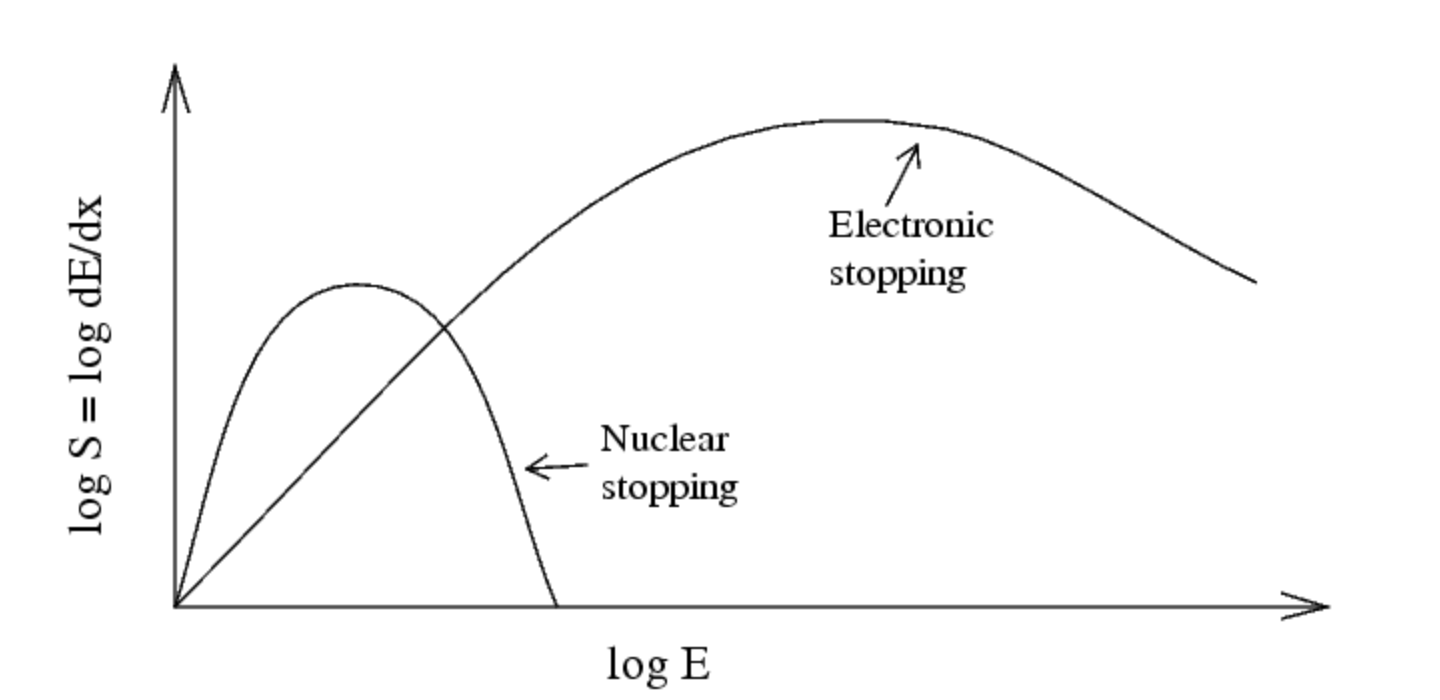
\includegraphics[width=0.6\linewidth, height=5cm]{ionstop2}
	\caption{Ratio between nuclear and electronic stopping power. The maximum of the nuclear stopping curve typically occurs at energies between 10--100 keV, of the electronic stopping power at MeV energies. For very light ions slowing down in heavy materials, the nuclear stopping is weaker than the electronic at all energies. \cite{4}}
	\label{fig:ionstop2}
\end{figure}

\subsection{Low Energy Regime}\label{subsec:low-energy-regime}
For $v < v_e$ we have a linear expression for $S_{ne}$.
There are several models to get this result, but all models converge to $S_{ne} \propto v$.
Two examples of these models are Firsov, where the ion loses a small amount of momentum if it picks up an electron, and the Linard-Scharff formula, which is written as with some pre-factor $K$ such that: $$S_{ne} \propto K \sqrt{E}$$
\subsection{High Energy Regime}\label{subsec:high-energy-regime}
At high energy, the ion is a bare nuclei and loses all of its electrons, and therefore has the pure coulomb potential from the target atoms.
Bohr calculates this classically, as the electron is basically not moving in comparison to the ion that flies by.
However, at high energies we must take into account the relativity effects, as well as the shell structure of the atom's electrons, and the QM effects.
This is called the Bethe-Bloch Formula.
The end results I write below, where first we see the Bohr expression for the electronic stopping power (classical)
\begin{equation}
	\frac{dE}{dx} \propto \frac{1}{E} \ln \frac{E}{E_B}\label{eq:borh}
\end{equation}
This is derived using a combination of Gauss law for a moving ion and stationary electron with Coulomb interaction to determine the change in momentum of the ion, and thus the change in energy.
and then the Bethe-Bloch Formula (including relativistic effects) for the electronic stopping power
\begin{equation}
	\frac{dE}{dx} = -\frac{Z_1^2 e^4 n_e}{4\pi \epsilon_0^2 v^2 m_e}\left[ \frac{1}{2} \ln \left( \frac{2m_e v^2 \gamma \Delta E_{max}}{I^2}\right) - \beta^2 - \frac{\delta}{2} - \frac{C}{Z_2}\right]\label{eq:beathe}
\end{equation}

\section{Summary}\label{sec:summary4}
The impact of ions on samples is quantified using \textit{stopping power}, which has components nuclear and electronic.
The ions can remain stuck in the sample because of this, and this stopping regime explains sputtering.
\begin{myitemize}
	\item As an ion penetrates a sample, there are different mechanisms that make the ion 'lose' energy as it collides with other atoms within the sample
	\item Nuclear stopping involves elastic collisions, and results in large discrete energy losses resulting in large angular deflection
	\item Electronic stopping involves inelastic collisions, and results in smaller energy loss per collision, thus negligible deflection.
	\item High energy electronic stopping is governed classically by coulomb potential, $S_{ne} \propto \left( \frac{Z_1}{v}\right)^2$, but exact solutions need to consider relativistic effects (Beathe-Bloch Formula)
	\item Low energy electronic stopping we have linear proportionality to velocity (thus $\propto \sqrt{E}$)
\end{myitemize}
